\chapter{RecercaPrevia}

\section{Què és la qualitat de l’aigua?}
La qualitat de l'aigua es un terme que es refereix a les caracteristicas fisicas, quimicas y bilogicas de l'aigua. Per determinar-la, s'analitzan alguns paràmetres.

Segons Wikipedia \cite{WikiAgua}, s'entén la qualitat de l'aigua com `característiques químiques, físiques, biològiques i radiològiques de l'aigua`, en relació amb necessitats humanes.

La Fundació Aquae \cite{Fundacionaquae} indica que es tracta d'un conjunt de paràmetres, com temperatura, contingut mineral i bacteris, mesurats i comparats amb estàndards, per definir si l'aigua és apta per a fins determinats o no.
\subsection{Tips de paràmetres per analitzar la qualitat de l'aigua}
\begin{enumerate}[1)]
 \item \textbf{Parametres químics}
 Relacionats amb la composició química de l’aigua; indiquen si és potable o contaminada.
 \begin{enumerate}[a)]
  \item \textit{pH}: Explicació a la secció \ref{subsec:ph}
  \item \textit{Duresa}: Explicació a la secció  \ref{subsec:duresa}
  \item \textit{Nitrats i Nitrits}: Explicació a la secció  \ref{subsec:nitratsnitrits}
  \item \textit{Clor (lliure i total)}: Explicació a la secció  \ref{subsec:clor}
  \item \textit{Metalls pesants}: Explicació a la secció   \ref{subsec:metallspesats}
 \end{enumerate}
 \item \textbf{Parametres físics}
 Mesuren característiques visibles o mesurables sense canviar la composició de l’aigua.
 \begin{enumerate}
  \item \textit{Temperatura}: Explicat a la secció \ref{subsec:temperatura}
  \item \textit{Color}: Explicat a la secció \ref{subsec:color}
  \item \textit{Olor i sabor}: Explicat a la secció \ref{subsec:olorisabor}
 \end{enumerate}
 \item \textbf{Parametres biologics}
 Indiquen la presència de microorganismes que poden ser patògens.
 \begin{enumerate}
  \item \textbf{Coliformes fecals}: Explicat a la secció \ref{subsec:coliformes}
  \item \textbf{Bacteris totals}: Explicat a la secció \ref{subsec:bacteris}
  \item \textbf{Algs i protozous}: Explicat a la secció \ref{subsec:algsiprotozous}
  \item \textbf{Índex biològic}: Explicat a la secció \ref{subsec:indexbiologic}

 \end{enumerate}

\end{enumerate}

\section{Explicació dels parametres químics}

\subsection{pH} \label{subsec:ph}
\subsubsection{Què és el pH?}
El pH és una mesura que serveix per establir el nivell d’acidesa o alcalinitat d'una dissolució. La `p` ve de `potencial` i l'`H` ve de l’àtom d’hidrogen, per això el pH és el potencial de l’hidrogen.

S'expressa com el logaritme negatiu de base 10 de la concentració de ions d'hidrogen: $ \text{pH} = -\log_{10} [\mathrm{H}^+] $.

A la fórmula la ${H}^+$ és la concentració de ions d'hidrogen en la solució, mesurat en mols per litre (mol/L). $-\log_{10}$ és el logaritme en base 10, el signe negatiu s'utilitza amb l'objectiu que el pH sigui un número positiu. La raó és perquè el logaritme d'un número menor que 1 és negatiu.

D'altra part, el \textbf{pOH} és una mesura de concentració de ions hidroxil ${OH}^-$ en una dissolució. S'expressa com el logaritme negatiu de base 10 de la concentració de ions hidroxil, i a diferència del pH, s'utilitza per mesurar el nivell d’alcalinitat d'una dissolució. Es calcula amb la formula  $ \text{pOH} = -\log_{10} [\mathrm{OH}^-] $.
\subsubsection{ Quina relació hi ha entre el nivell d'acidesa i el pH?}
Les dissolucions àcides tenen una alta quantitat de ions d'hidrogen. Això significa que tenen baixos valors de pH, i per tant, el seu nivell d'acidesa és elevat. Així que una dissolució serà més o menys àcida depenent de la quantitat d'hidrogen que contingui aquesta.

D'altra banda, les dissolucions bàsiques (alcalines) tenen baixes quantitats de ions d'hidrogen. Això vol dir que tenen alts valors de pH, i per tant el seu nivell d'acidesa és baix.
\subsubsection{Escala del pH}
\begin{figure}[h!]
\centering
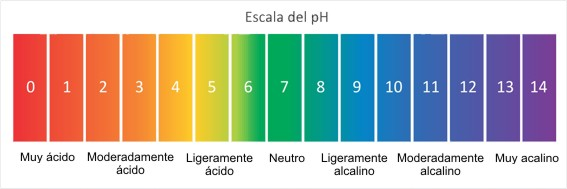
\includegraphics[width=0.9\textwidth]{./Figures/EscaladepH.png}
\caption{Escala del pH}
\label{fig:escaladeph}
\end{figure}
L'escala de pH s'utilitza per mesurar el grau d'acidesa d'una dissolució, i com que el pH està relacionat amb el pOH, coneixent el grau d'acidesa d'una dissolució, també podem saber el seu grau d'alcalinitat (basicitat).

Com podem observar a la figura \ref{fig:escaladeph}, el valor del pH va del 0 al 14. Les substàncies amb pH igual a 0 són més àcides; les que tenen el pH = 7 són neutres, i les que tenen pH = 14 són les menys àcides, per tant, són les més bàsiques.

\subsubsection{Què ens diu el pH sobre la qualitat de l'aigua?}
El pH és un paràmetre fonamental entre els paràmetres; com he dit abans, indica el grau d'acidesa o alcalinitat. El pH depèn de la quantitat d'hidrogen que conté l'aigua.

Un pH d'1 ens diu que la substància és molt àcida i, per tant, perillosa. L'àcid clorhídric (HCl(aq)) té aproximadament aquest pH. A l'altre extrem de l'escala, amb un pH aproximat de 14, tenim sosa càustica (NaOH). Gràcies a l'escala de pH (figura \ref{fig:escaladeph}), podem saber si la dissolució és més àcida o bàsica. En general, un pH de 7, és a dir, neutre, seria el més òptim en la majoria dels casos; és un pH similar al del nostre cos, la suor, etc.
\subsection{Duresa} \label{subsec:duresa}
\subsubsection{Què és la duresa de l'aigua?}
Es la concentració de compostos minerals en una certa quantitat d'aigua, especialments sals de magnesi i calci \cite{Facsa}. L'aigua `dura` te una alta concentracio d'aquestes sals i l'aigua `suau`, te una concentracio baixa d'aquestes. La duresa es pot calcular amb la seguennt formula: (mg/L de Calci (Ca) + mg/L de Magensi (Mg) x 4.2 )/10
\subsubsection{Com t’afecta la duresa de l’aigua?}
L'Organització Mundial de la Salut no considera que la duresa de l'aigua tingui un impacte negatiu en l'organisme . En una guia, afirma que els paràmetres per al consum oscil·len entre 100 i 300 mg/l de carbonat de calci, encara que el llindar de tolerància pot estar per sobre o per sota en funció de la normativa de cada país. \cite{Brita}

En general, la concentració desitjable es considera inferior a 100 mg/l (aigua de més qualitat) i que per sobre de 500 mg/l qualitat ja no és acceptable. En el cas concret d'Espanya, la normativa tecnicològica-sanitària estableix un valor de contingut de calci de fins a 100 mg/l amb un límit màxim de tolerància de 200 mg/l. \cite{Brita}
\subsection{Nitrats i Nitrits} \label{subsec:nitratsnitrits}
\subsubsection{Què són els nitrat i el nitrit?}
El nitrat \(\mathrm{NO_3^-}\) és un compost químic format bàsicament per nitrogen i oxigen. Naturalment es troba en el sòl i l'aigua, per la qual cosa és un nutrient fonamental per a molts éssers vius.

Quan paguem la terra per millorar el seu rendiment, utilitzem productes de nitrogen, ja siguin fertilitzants minerals o orgànics com els fems. A aquest augment de nitrats, hem d'afegir el plus que representa nitrogen contingut en aigua de reg (aigua utilitzada per el reg de conreus o jardins). Per tant, el nivell final d'aquest compost pot ser alt en moltes ocasions.

Amb el temps, i essencialment a causa de l'acció d'alguns bacteris, aquests nitrats evolucionen en nitrits \(\mathrm{NO_2^-}\), ions considerats més tòxics.
\subsubsection{El nitrit i les seves conseqüències}
El nitrit s'origina en les fruites profundes que es produeixen quan el sistema de reg mou el nitrat al sòl. Aquest risc és més alt quan s'utilitza el reg de la superfície. La contaminació de l'aigua superficial pot tenir conseqüències tan greus com la mort de la fauna aquàtica a llarg termini.

Com hem vist, l'excés de nitrit pot causar la seva contaminació a l'aigua, però també als cultius que estan regats amb aquesta aigua contaminada. Per tant, moltes verdures es poden veure afectades.

Aquestes grans quantitats de nitrits a l'aigua poden tenir un impacte negatiu en la salut de les persones. Per evitar problemes, l'OMS recomana un límit de 50 mil·ligrams de nitrat per litre. \cite{OMS}
\subsection{Clor} \label{subsec:clor}
\subsubsection{Què és el clor i quina relació te amb l'aigua?}
El clor és un element químic, un gas groc verdós, dens i amb una olor irritant. S'utilitza principalment per desinfectar l'aigua, eliminant així les bacteris i altres microorganismes nocius.

La seva presència és considerada l'últim pas per a la potabilització de l'aigua. Desinfecta microorganismes patògens que causen malalties als humans; per aquesta raó, la seva desinfecció és fonamental en la protecció de la salut pública.

Tot i que existeixen altres mètodes de desinfecció, el clor ha sigut el responsable de l'augment de l'esperança de vida a l'Europa del passat segle XX. Però, anteriorment, fa cinc segles, s'utilitzaven altres formes de desinfecció més rudimentàries, com bullir l'aigua.

La revista Life \cite{RevistaLife} classifica el logre de la cloració (procés de desinfecció que utilitza clor) com “probablement el més significatiu progrés de la salut pública del mil·lenni” l'any 1997.

Per tant, el clor és un producte químic amb l'objectiu de desinfectar l'aigua. Tanmateix, l'ús d'aquest component químic \textbf{no és segur.}
\subsubsection{Com el clor de l'aigua potable afecta la salut}
Segons el doctor en Medicina Josep Lluís Berdonces, qui es basa en diferents estudis sobre aquest tema, la cloració de l’aigua pot tenir efectes nocius sobre la salut de les persones. Té en la seva composició àcids húmics i fúlvics. Les conseqüències d’aquests components químics sobre la salut humana són variades. Molts d’ells tenen una gran afinitat per unir-se amb els diversos greixos del cos. \cite{Clor}
\subsection{Metalls pesants} \label{subsec:metallspesats}
\subsubsection{QQuè són els metalls pesants a l’aigua?}
El terme de `metalls pesants` es refereix a qualsevol element químic metàl·lic que té una alta densitat i pot ser tòxic o verinós a baixes concentracions.

Alguns metalls pesants com el coure ($Cu$), el seleni ($Se$), i el zinc ($Zn$) són essencials per mantenir el metabolisme del cos humà. No obstant això, en altes quantitats poden conduir a l'enverinament. Aquesta intoxicació pot ocórrer si es consumeix aigua amb algun d’aquests metalls.
\subsubsection{Com es contamina l’aigua amb metalls pesants?}
El principal motiu és la contaminació industrial. Una altra font de contaminació pot ser els abocaments d'aigües residuals. Hi ha casos en què l’aigua pateix un procés d’enriquiment de metalls pesants, ja que passa per roques que contenen aquests metalls en la seva composició.
\subsubsection{Metalls pesants presents a l'aigua}
\begin{enumerate}
 \item \textit{\textbf{Alumini}}
 Tot i que l'alumini no és un metall pesat, representa aproximadament el 8 per cent de la superfície terrestre i és el tercer element més abundant. Està disponible per a la ingestió humana a través de l'aigua potable.
 \item \textit{\textbf{Arsènic}}
 L'arsènic és la causa més freqüent d'enverinament per metalls pesants aguts en adults. L'arsènic també es pot trobar en el subministrament d'aigua, el que porta a l'exposició en marisc, bacallà, haddock i alguns altres aliments marins
 \item \textit{\textbf{Coure}}
 El coure a altes concentracions pot ser tòxic. Els efectes per a la salut són els següents: pot causar vòmits, diarrea, pèrdua de força o, per a l'exposició severa, la cirrosi del fetge.
 \item \textit{\textbf{Ferro}}
 El ferro és un metall pesant comú a l'aigua, s'ha de tenir cura de menjar suplements de ferro, i en la dieta pot enverinar agudament els nens petits. La ingestió representa la major intoxicació per ferro per a les persones.
 \item \textit{\textbf{Mercuri}}
 El mercuri es genera naturalment en el medi ambient en la desgasificació de l'escorça terrestre i les emissions volcàniques.
\end{enumerate}
\textit{\textbf{NOTA}}: Tota aquesta informació l'he trobada a la web de Carbotecnia \cite{Carbotecnia}
\section{Explicació dels parametres físics}

\subsection{Temperatura} \label{subsec:temperatura}
La temperatura és un paràmetre físic que permet mesurar les sensacions de calor o fred. En termes científics, és una mesura de l’energia cinètica de les molècules que el componen, és a dir, com de molt es mouen o s’agiten aquestes molècules.
\subsubsection{Quina relació te amb la qualitat de l'aigua?}
Un gran exemple de la importància de la temperatura és a la vida aquàtica. Per exemple, l’aigua freda reté més oxigen; això fa que sigui vital per als peixos i altres éssers aquàtics. Quan aquesta temperatura augmenta, la quantitat d’oxigen disminueix, afectant així la supervivència d’aquests organismes.

També afecta el metabolisme dels organismes: els animals aquàtics i les plantes tenen un rang de temperatura ideal. Si aquest rang és superat per molt de temps, els organismes poden patir malalties o fins i tot aquest canvi pot portar-los a la mort.

Una dada curiosa és que, a temperatures més altes, algunes substàncies tòxiques es tornen més actives o més perilloses per als organismes.
\subsection{Color} \label{subsec:color}

\subsection{Olor i sabor} \label{subsec:olorisabor}

\section{Explicació dels parametres biologics}

\subsection{Coliformes fecals} \label{subsec:coliformes}

\subsection{Bacteris totals} \label{subsec:bacteris}

\subsection{Algs i protozous} \label{subsec:algsiprotozous}

\subsection{Índex biològic} \label{subsec:indexbiologic}


